\documentclass[tikz,border=5pt]{standalone}
\begin{document}
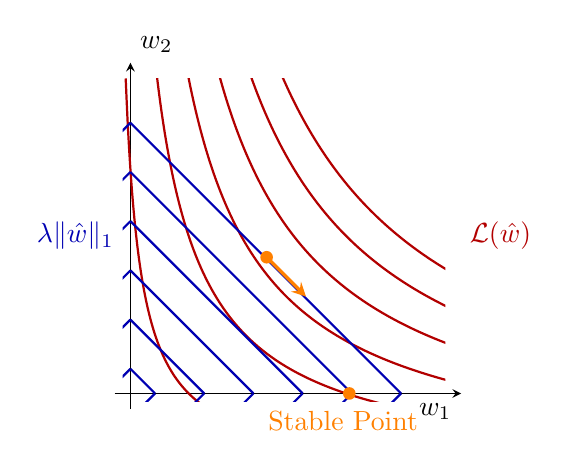
\begin{tikzpicture}[scale=1.0,>=stealth]
  % 坐标轴
  
  \draw[->] (-0.2,0) -- (4.2,0) node[below left] {$w_1$};
  \draw[->] (0,-0.2) -- (0,4.2) node[above right] {$w_2$};
  \begin{scope}
    \clip (-0.1,-0.1)rectangle(4,4);

  % 用 foreach 画多条反比例函数
  \foreach \k in {1,3,...,11}{

    \draw[domain=0.2:5,  samples=200, smooth,thick,red!70!black]
      plot (\x-0.26,{\k/\x-1});
    \draw[thick,blue!70!black]
      (\k/3.2,0)--(0,\k/3.2);
      \draw[thick,blue!70!black]
      (\k/3.2,0)--(0,-\k/3.2);
    \draw[thick,blue!70!black]
      (-\k/3.2,0)--(0,\k/3.2);
    \draw[thick,blue!70!black]
      (-\k/3.2,0)--(0,-\k/3.2);
  }
    
  \end{scope}
  \node[blue!70!black,thick] 
  at(-0.7,2) {$\lambda\|\hat w\|_1$};
  \node[red!70!black,thick] at(4.7,2) {$\mathcal L(\hat w)$};
  \fill[orange] (1.73,1.73) circle (0.08);
  \fill[orange] (2.78,0) circle (0.08);
\node[orange,thick] at(2.7,-0.35) {Stable Point};
  \draw[->,very thick,orange] (1.73,1.73) --++(0.5,-0.5);
\end{tikzpicture}
\end{document}